Táto kapitola slúži na popísanie teórie, poznatkov a metód, ktorými sme sa inšpirovali alebo nám pomohli pri vypracovávaní témy zadania.
\section{CRISP-DM}
CRISP-DM je metodológia pre vyjadrenie životného cyklu získavania dát, ktorý bol vytvorený konzorciom NCR, SPSS a Daimler-Benz. Tento formát definuje hierarchiu skladajúcu sa z hlavných fáz, bežných i špecializovaných úkonov až po inštancie procesu. Hlavnými fázami tejto metodológie sú:\par
\begin{enumerate}
  \item Porozumenie cieľom z businesového hľadiska - určenie cieľov získavania dát, zistenie potrebných okolností vo firme, špecifikácia.
  \item Porozumenie dátam - získanie a integrácia potrebných dát
  \item Príprava/Predspracovanie dát - čistenie, transformácia, redukcia šumu ...
  \item Modelovanie - voľba algoritmov, architektúry a predpokladov, tvorba a testovanie modelov
  \item Evaluácia - zistenie presnosti predikcií, skrytých chýb, splnenia cieľov
  \item Spustenie do prevádzky - zabezpečenie funkčnosti a údržby, zhodnotenie
\end{enumerate}
Tieto fázy znázorňuje obrázok \ref{img:crisp-dm}. Postupnosť týchto fáz nie je napevno zadefinovaná. Pohybovanie sa medzi fázami dopredu čí dozadu je vždy potrebné. Výsledok každej fázy predurčuje ktorá fáza alebo ktorý úkon danej fázy sa má vykonať ďalej. Jednotlivé fázy si rozoberieme podrobnejšie v ďalšej časti.
\begin{figure}[H]
	\begin{center}
		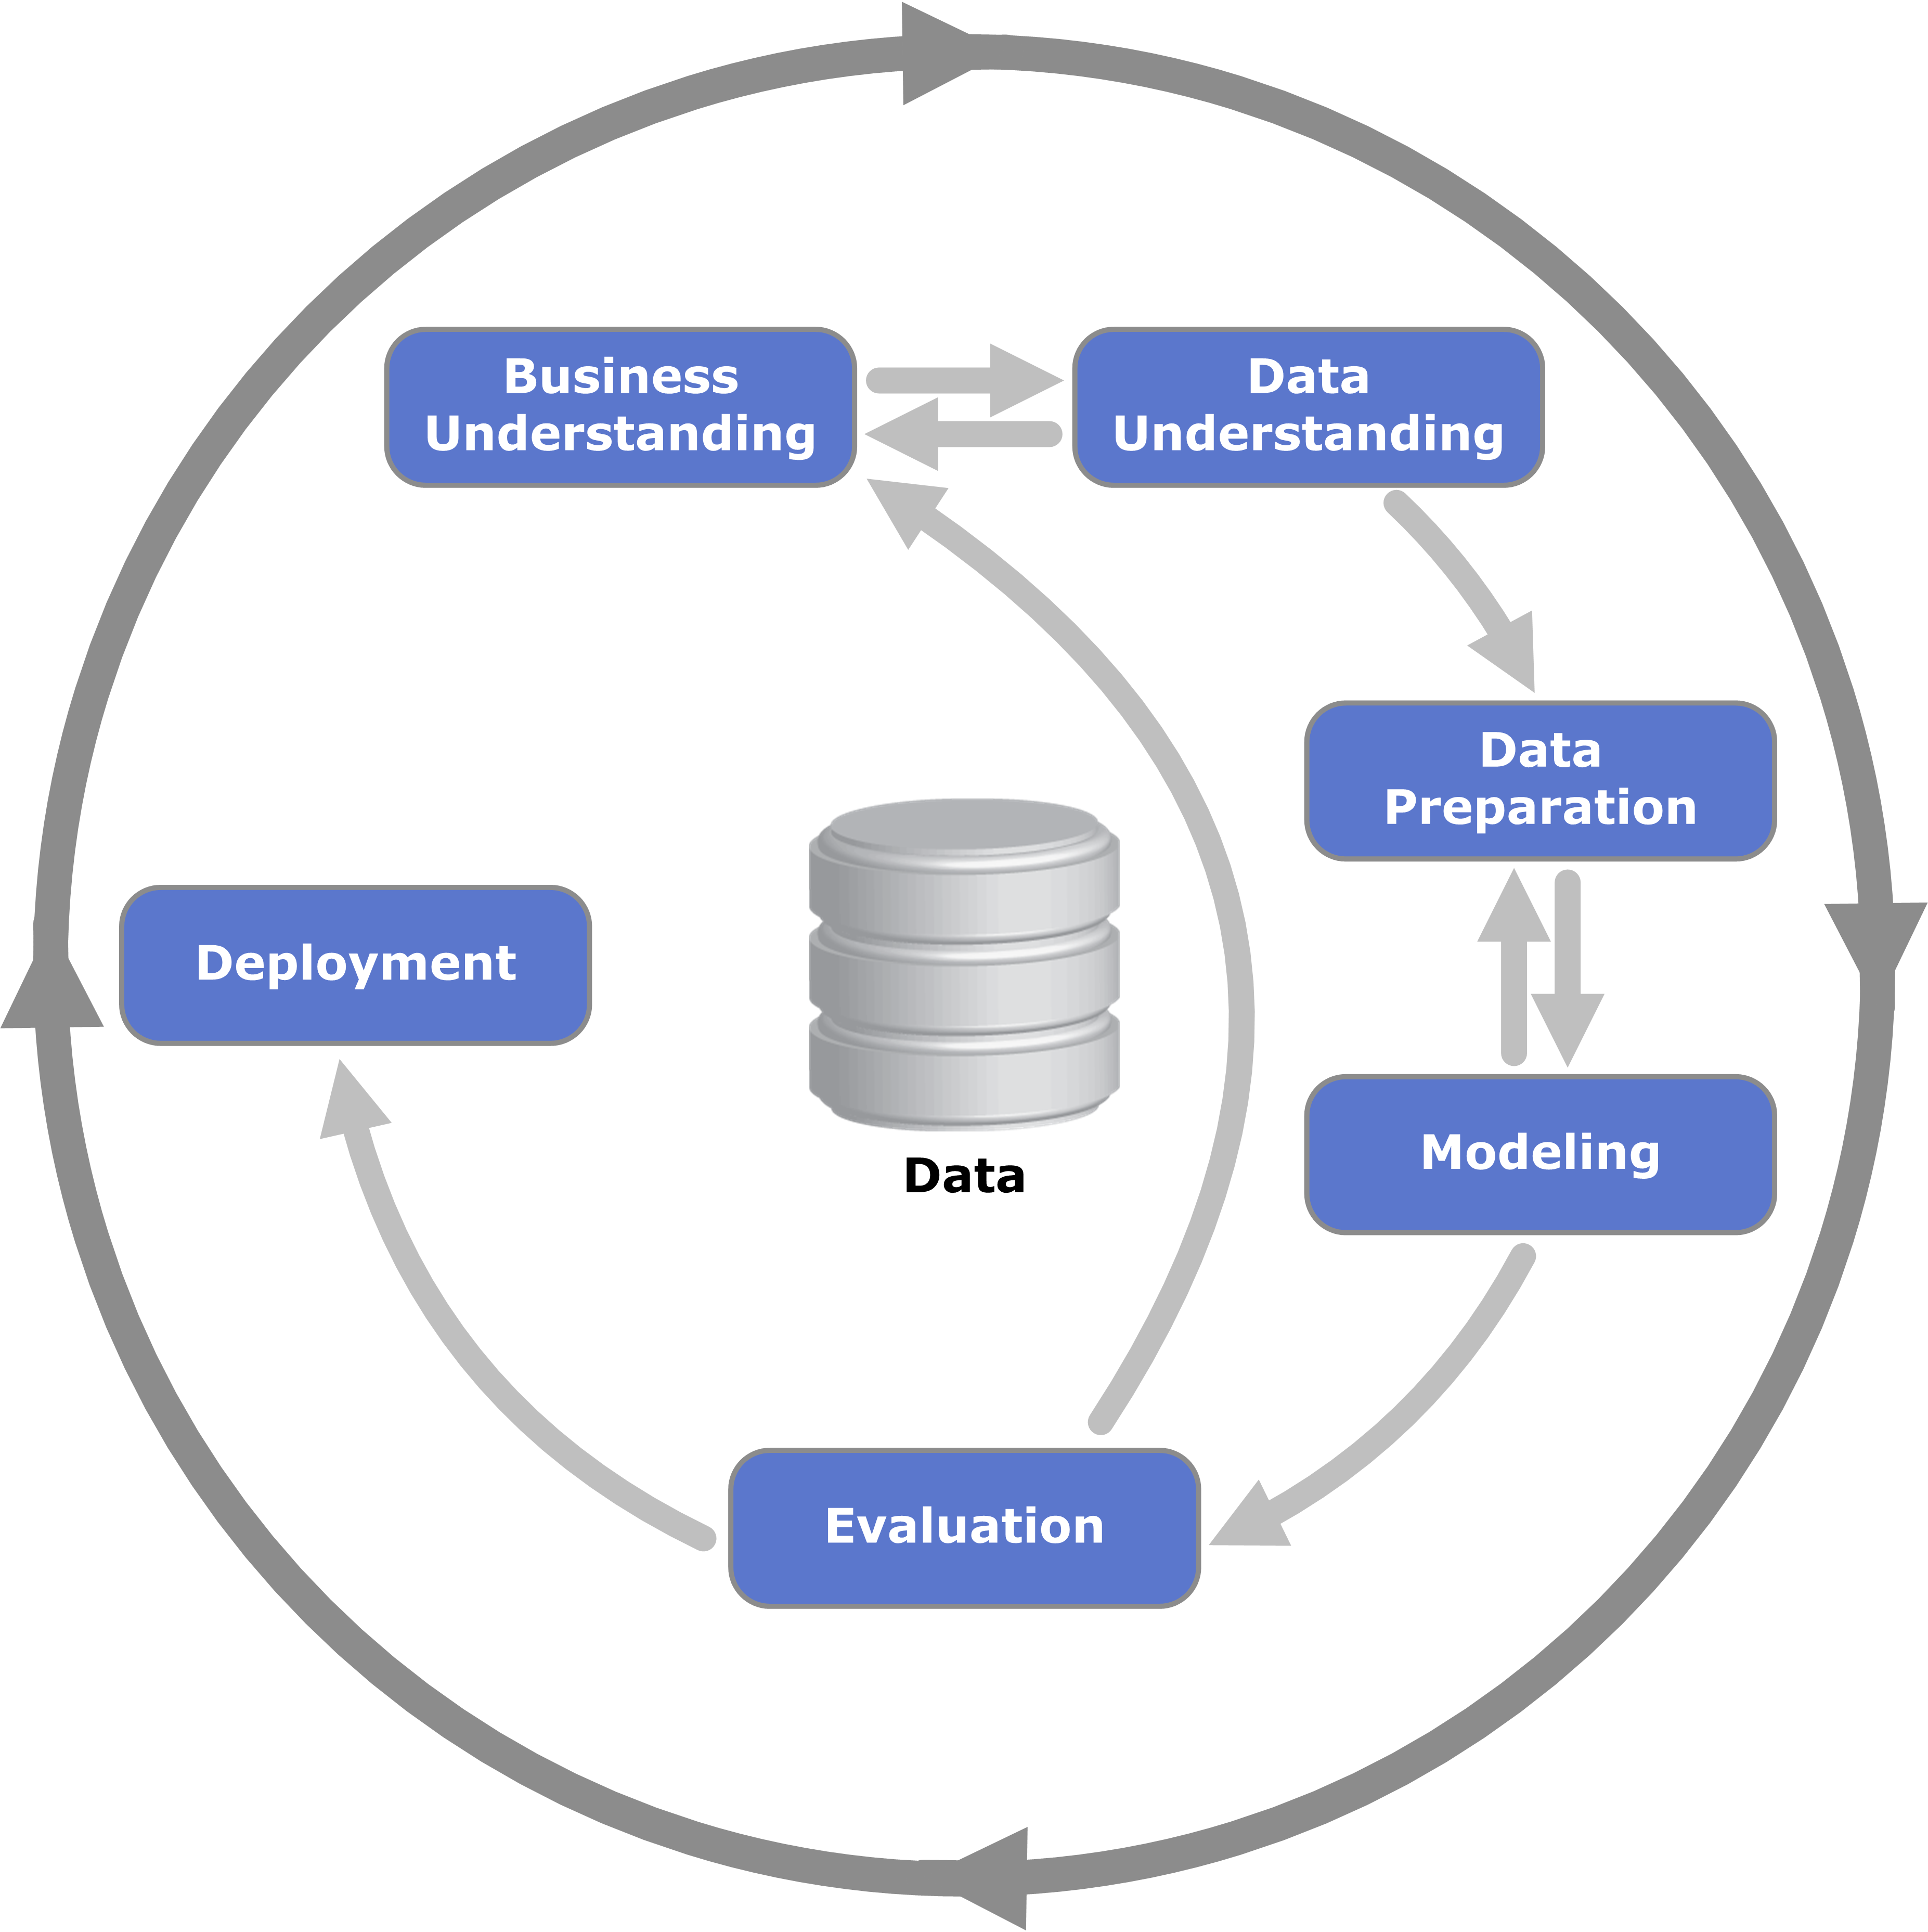
\includegraphics[scale=0.6]{img/crisp-dm.png}
		\caption{Fázy formátu CRISP-DM}
		\label{img:crisp-dm}
	\end{center}
\end{figure}
\subsection{Porozumenie cieľom}
Úvodná fáza sa zameriava na porozumenie cieľov a požiadaviek daného projektu z businesového hľadiska, následne sa využíva toto porozumenie na vytvorenie problému získavania dát a prvorného plánu ako dosiahnuť dané cieľe.
\subsection{Porozumenie dátam}
Fáza porozumenia dát začína zhromažďovaním dát a pokračuje aktivitami, ktoré nám umožňujú zoznámiť sa so získanými dátami, identifikovať problémy kvality dát, objaviť prvé poznatky z dát a taktiež detekovať zaujímavé podmnožiny na vytvorenie hypotéz ohľadom skrytých informácii.
\subsection{Príprava dát}
Príprava dát zahŕňa všetky aktivity potrebné na vytvorenie konečnej dátovej množiny z počiatočných surových dát. Úlohy prípravy dát sú častokrát uskutočňované viac krát a nemajú danú postupnosť. Takéto úlohy sú napr. selekcia tabuliek, záznamov a atribútov ako aj transformácie a čistenie dát pre modely ktoré chceme využívať. 
\subsection{Modelovanie}
V tejto fáze sa vyberajú a uplatňujú rôzne modelovacie techniky a experimenty s ich parametrami pre optimálne fungovanie. Zvyčajne existuje viacero techník pre ten istý problém získavania dát. Niektoré techniky vyžadujú špecifické požiadavky na formu v ktorej sú dáta uložené. A teda vrátenie sa do predchádzajúcej fázy je častokrát nevyhnutné.
\subsection{Evaluácia}
V tomto stave projektu už máme vytvorený model, ktorý sa zdá, že je vysokej kvality z perspektívy dátovej analýzy. Predtým ako uvedieme daný projekt do prevádzky je dôležité ho dôkladne evaluovať a zrevidovať kroky, ktoré boli uskutočnené na jeho vytvorenie, aby sme si boli istý, že model spĺňa businesové ciele. Kľúčovým cieľom je zistiť, či existuje nejaký dôležitý cieľ, ktorý nebol dostatočne zahrnutý v procese. Na konci tejto fázy by sme mali dôjsť k výslednému použitiu výsledkov získavania dát.
\subsection{Spustenie do prevádzky}
Vytvorenie modelu častokrát neznačí koniec projektu. Aj keby účelom modelu bolo len lepšie porozumenie dátam, toto porozumenie je treba zorganizovať a odprezentovať tak aby ho klienti mohli efektívne využiť. V závislosti na požiadavkách projektu, fáza spustenia do prevádzky môže byť jednoduchá ako napr. len vytvoriť správu o výsledkoch ale aj zložitá ako napr. implementácia opakovateľného získavania dát v celom podniku. Kroky tejto fázy vykonáva najmä klient. Napriek tomu ak uvádzanie do prevádzky vykonáva analytik je dôležité aby klient vopred pochopil aké úkony je potrebné vykonať na správne využitie vytvorených modelov.
\section{Hĺbková analýza dát}
Hĺbková analýza dát (data mining) je metodológia na riešenie problémov, ktorá snaží nájsť logický alebo matematický opis vzorcov a závislostí v dátových množinách. Existujú dve základné metódy ako sa dá vykonávať hĺbková analýza dát. Sú to metódy strojového učenia: učenie s učiteľom a učenie bez učiteľa. Tieto techniky v kontexte hĺbkovej analýzy dát majú vykonávať dve dôležité úlohy:
\begin{enumerate}
  \item Generalizovať z množiny známych príkladov.
  \item Podrobne popisovať štruktúru dát.
\end{enumerate}
\par Hĺbková analýza dát umožňuje produkovať vedecké vedomosti v oboroch, ktoré nie sú ešte vhodné na tradičny matematický prístup. Norman Packard ukázal v \cite{6} a \cite{7} ako algoritmy učenia a optimizácie môžu byť použité na produkovanie optimálnych modelov z experimentálnych dát napriek absencii predošlých teoretických vysvetlení. Vedomosti získané tymito metódami boli aplikované na velké množstvo rôznych domén napr. chémia, predaj, bankovníctvo a veda.
\section{Strojové učenie}
Existuje mnoho uplatnení pre strojové učenie, jedným z najdôležitejších je hĺbková analýza dát (data mining). Ľudia sú často náchylný na robenie chýb počas analyzovania dát alebo keď sa snažia určiť vzťahy medzi veľkým množstvom charakteristík. Táto skutočnosť spôsobuje ľudom ťažkosti pri nachádzaní riešenia pre rôzne problémy. Strojové učenie vieme mnohokrát aplikovať na takéto problémy, čím sa zvyšuje efektivita systémobv a návrh mašín.\par
Každý príklad v učitej dátovej množine použitý niektorým z algoritmov strojového učenia je reprezentovaný použitím rovnakej množiny chrakteristík. Tieto charakterisktiky môžu byť binárne, spojité alebo kategorické. Ak sú príklady dodané aj so známymi označeniami (správny korešpondujúci výstup) tak takéto učenie voláme učenie s učiteľom. Na druhej strane máme prípad kedy tieto označenia nepoznáme a teda ide o učenie bez učiteľa.
\section{Učenie bez učiteľa}
V tejto časti si povieme niečo o technikách strojového učenia bez učiteľa. Tieto techniky uľahčujú analýzu surových dat, čiže nám pomáhajú generovať analytické náhľady z neoznačených dát. Učenie bez učiteľa má veľa aplikácií ako napríklad detekcia charakteristík, dátové zhlukovanie, redukcia dimenzie, detekcia anomálií atď. Najnovšie posunutia v hierarchickom učený, zhlukovacích algoritmoch, analýzy faktorov a detekcie outlierov výrazne pomohli posunúť súčasný stav techniky učenia bez učiteľa.\par
Učenie bez učiteľa sa častokrát používa v kombinácii s učením s učiteľom kedy ide o takzvané učenie s čiastočným učiteľom. Táto technika nám pomáha predspracovať dáta pred ich analyzovaním a teda uľahčuje vytváranie dobrej reprezentácie charakteristík ako aj hľadanie vzorov a štruktúr v neoznačených dátach.
Na obrázku \ref{img:bez_ucitela} môžeme sledovať taxonómiu učenia bez učiteľa.
\begin{figure}[H]
	\begin{center}
		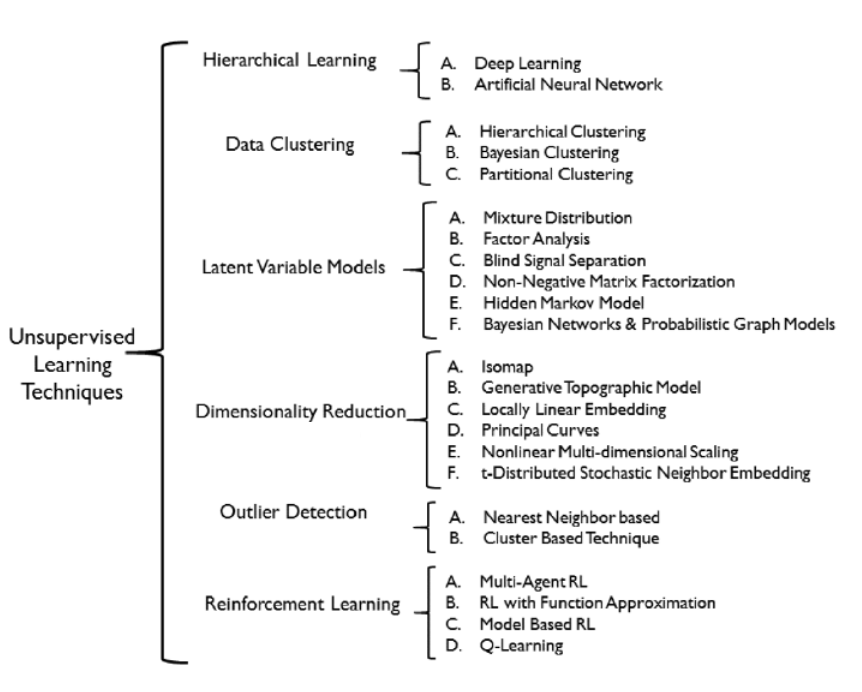
\includegraphics[scale=0.6]{img/tax_bez_ucitela.png}
		\caption{Taxonómia techník učenia bez učiteľa}
		\label{img:bez_ucitela}
	\end{center}
\end{figure}
\subsection{Zhlukovanie dát}
V našej práci z techník učenia bez učiteľa využívame najmä techniku zhlukovania dát, preto si algoritmy z tejto techniky viac priblížime.\par
Zhlukovanie dát je technika, ktorá má za účel nájsť skryté vzory v neoznačených vstupných dátach vo forme zhlukov \cite{zhluk_basic}. Jednoducho povedané táto technika sa snaží obsiahnuť usporiadanie dát v zmysluplných prirodzených zoskupeniach na základe podobnosti medzi rôznymi charakteristikami na naučenie sa o ich štruktúre. Zhlukovanie produkuje organizáciu dát takým spôsobom, že existuje vysoká podobnosť vrámci jedného zhluku a zároveň nízka podobnosť medzi zhlukmi. Výsledné štrukturované dáta sa nazývajú dátový koncept \cite{data_concept}. Táto technika má početne veľa aplikácii v rôznych oblastiach ako napr. strojové učenie, hĺbková analýza dát, analýza sietí, rozpoznávanie vzorcov a počítačové videnie.\par
Krátky prehľad rôznych typov zhlukovacích metód a ich vzťah môžme vidieť na obrázku \ref{img:zhluk}. Zhlukovanie môžeme rozdeliť na tri hlavné typy a to hierarchické zhlukovanie, Bayesovské zhlukovanie a čiastkové zhlukovanie. Hierarchické zhlukovanie vytvára hierarchickú dekompozíciu dát. Bayesovské zhlukovanie tvorí pravdepodobnostný model dát, ktorý rozhoduje o zaradení nového testovacieho bodu pravdepodobnostne. Naopak čiastkové zhlukovanie konštruuje viacero častí a vyhodnotí ich na základe nejakého dopredu určeného kritéria alebo charakteristiky ako napr. Euklidovská vzdialenosť.\par
V našej práci z týchto techník budeme hlavne využívať algoritmy hierarchického a čiastkového zhlukovania.
\begin{figure}[H]
	\begin{center}
		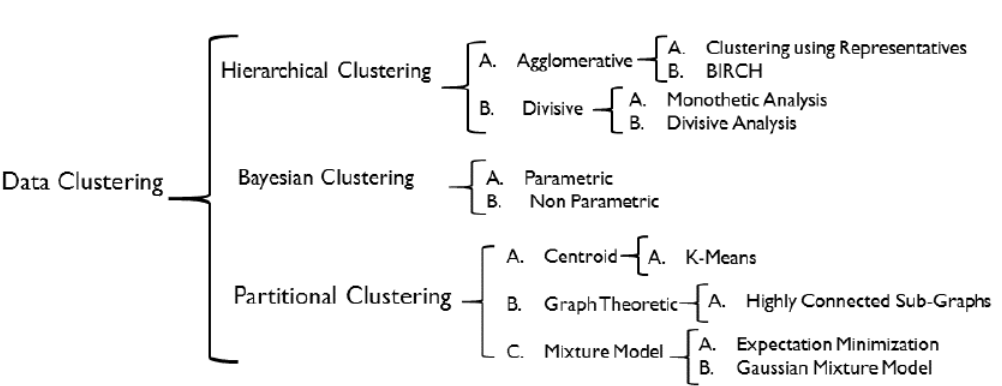
\includegraphics[scale=0.55]{img/tax_zhluk.png}
		\caption{Taxonómia techník zhlukovania dát}
		\label{img:zhluk}
	\end{center}
\end{figure}
\subsubsection{K-means zhlukovanie}
Zhlukovanie K-means je jednoduchý ale za to široko využiteľný prístup používaný na úlohu klasifikácie. Na vstup očakáva štatistický vektor, ktorý využije na dedukciu klasifikačných modelov či klasifikátorov. K-means zhlukovanie má tendenciu distribuovať \textit{m} pozorovaní do \textit{n} zhlukov, kde každé pozorovanie patrí k najbližšiemu zhluku. Patričnosť nejakého pozorovania do zhluku je určená pomocou priemeru alebo stredu zhluku. Tento algoritmus je používaný v mnohých aplikáciach v oblasti strojového učenia a hĺbkovej analýzy dát.\par
Obrázok \ref{img:k_means} názorňne zobrazuje výsledok K-means zhlukovania, kde môžme vidieť jednotlivé zhluky ako aj ich centroidy.
\begin{figure}[H]
	\begin{center}
		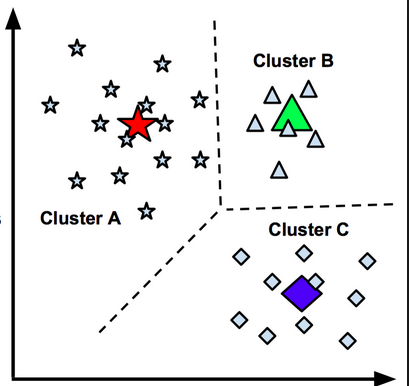
\includegraphics[scale=0.55]{img/k_means.png}
		\caption{Ukážka K-means zhlukovania}
		\label{img:k_means}
	\end{center}
\end{figure}
Jednou z variácií K-means algoritmu je algoritmus K-medoids. V tejto variácii algoritmu sa namiesto stredu zhluku využívajú dátové body, ktoré sú lokalizované najviac v strede korešpondujúceho zhluku.
\subsubsection{Hierarchické zhlukovanie}
Hierarchické zhlukovanie je veľmi známa stratégia využívaná v oblasti hĺbkovej analýzy dát a štatistickej analýzy, v ktorej sú dáta zhlukované do hierarchií zhlukov použitím aglomeratívneho (zdola hore) alebo rozdelujúceho (zvrchu nadol) príncípu. Skoro všetky algoritmy hierarchického zhlukovania sú bez učiteľa a deterministické. Na obrázku \ref{img:hierarch} môžeme sledovať hierarchickú štruktúru zhlukov, ktorá sa vytvára pri použití tohto algoritmu. \par
\begin{figure}[H]
	\begin{center}
		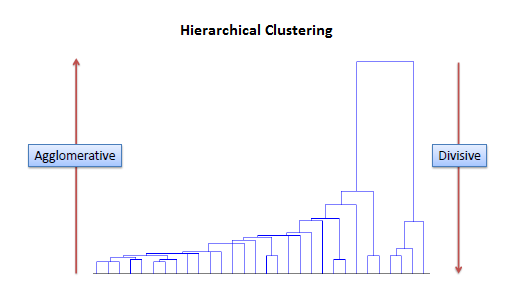
\includegraphics[scale=0.6]{img/hierarchical.png}
		\caption{Ukážka hierarchického zhlukovania.}
		\label{img:hierarch}
	\end{center}
\end{figure}
Hlavnou výhodou tejto techniky oproti K-means algoritmu je skutočnosť, že táto technika nepotrebuje mať dopredu špecifikovaný počet zhlukov. Avšak táto výhoda má za cenu výpočtovú náročnosť. Bežné algoritmy hierarchického zhlukovania majú aspoň kvadratickú výpočtovú časovú zložitosť v porovnaní s lineárnou výpočtovou časovou zložitosťou K-means algoritmu.\par
Metódy hierarchického zhlukovania majú aj svoje nevýhody. Tieto metódy zlyhávajú v presnej klasifikácii zašumených vysoko-rozmerných dát, kde ich heuristika môže zlyhať kvôli štrukturálnym nepresnostiam empirických dát. Okrem toho, výpočtová časová zložitosť bežných aglomeratívnych hierarchických algoritmov je NP-ťažká.
\section{Učenie s učiteľom}
Táto časť slúži na priblíženie techník a algoritmov učenia s učiteľom, ktoré využívame v našej práci. Učenie s učiteľom je kategória problémov strojového učenia kedy poznáme požadovaný výsledok ku každému trénovaciemu príkladu.\par
Hlavné dve úlohy učenia s učiteľom su klasifikácia a regresia. Ak požadovaný výsledok pri trénovacích príkladoch má hodnotu spojitého charakteru tak ide o problém regresie. Na druhej strane máme prípady kedy požadované výsledky pre trénovacie príklady nadobúdajú hodnoty z diskrétnej konečnej množiny, vtedy ide o klasifikáciu \cite{Goodfellow-et-al-2016}. V našej práci využívame z kategórie učenia s učiteľom využívame algoritmy klasifikácie.
\subsection{Proces učenia}
Napriek veľkým rozdielom medzi jednotlivými algoritmami učenia s učiteľom, proces učenia vieme generalizovať. Obrázok \ref{img:super_process} popisuje proces učenia pre algoritmi učenia s učiteľom.\par
\begin{figure}[H]
	\begin{center}
		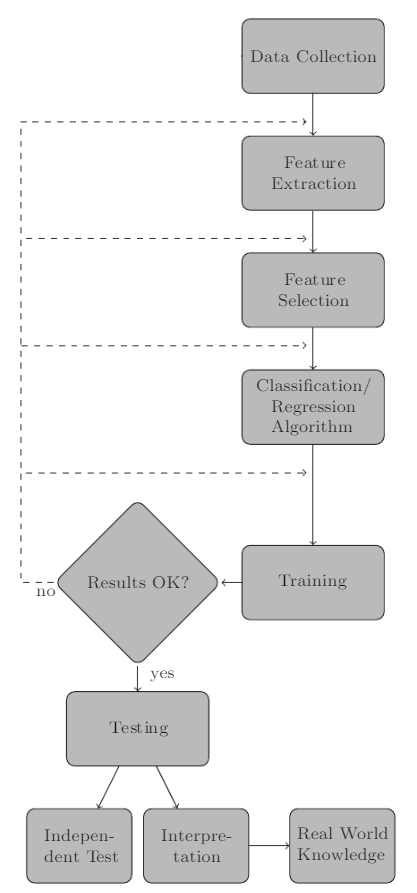
\includegraphics[scale=0.5]{img/supervised_process.png}
		\caption{Proces učenia pri metóde učenia s učiteľom.}
		\label{img:super_process}
	\end{center}
\end{figure}
Proces začína zbieraním dát o danom probléme, ktorý chceme riešiť. Po úpešnom zozbieraní dát je potrebné z dát získať charakteristiky. Potom potrebujeme vybrať dôležité charakteristiky pre náš konkrétny problém. Keď už máme takto pripravené dáta, môžeme použiť niektorý z modelov strojového učenia podľa druhu úlohy či klasifikácie alebo regresie. Po natrénovaní modelu je potrebné model evaluovať. Tu sa proces rozvetvuje ako sú výsledky evaluácie nedostatočné, tak sa musíme vrátiť ku niektorému z predošlých krokov. Ak evaluácia dopadla úspešne tak sa model otestuje na novej nezávislej množine a následne sa môže použiť na extrahovanie vedomostí z reálneho sveta.
\subsection{Rozhodovacie stromy}
Rozhodovanie stromy sú stromy, ktoré klasifikujú príklady pomocou utriedenia ich na základe hodnôt atribútov. Každý vrchol rozhodovacieho stromu reprezentuje nejaký atribút v príklade, ktorý chceme klasifikovať. Každá hrana rozhodovacieho stromu reprezentuje hodnotu, ktorú vrchol ku ktorému prislúcha môže nadobudnúť. Príklady sú klasifikované tak, že začínaju v koreni stromu a sú triedené na základe hodnôt jednotlivých atribútov, ktoré nadobúdajú. Obrázok \ref{img:decision_tree} znázorňuje príklad takéhoto rozhodovacieho stromu.
\begin{figure}[H]
	\begin{center}
		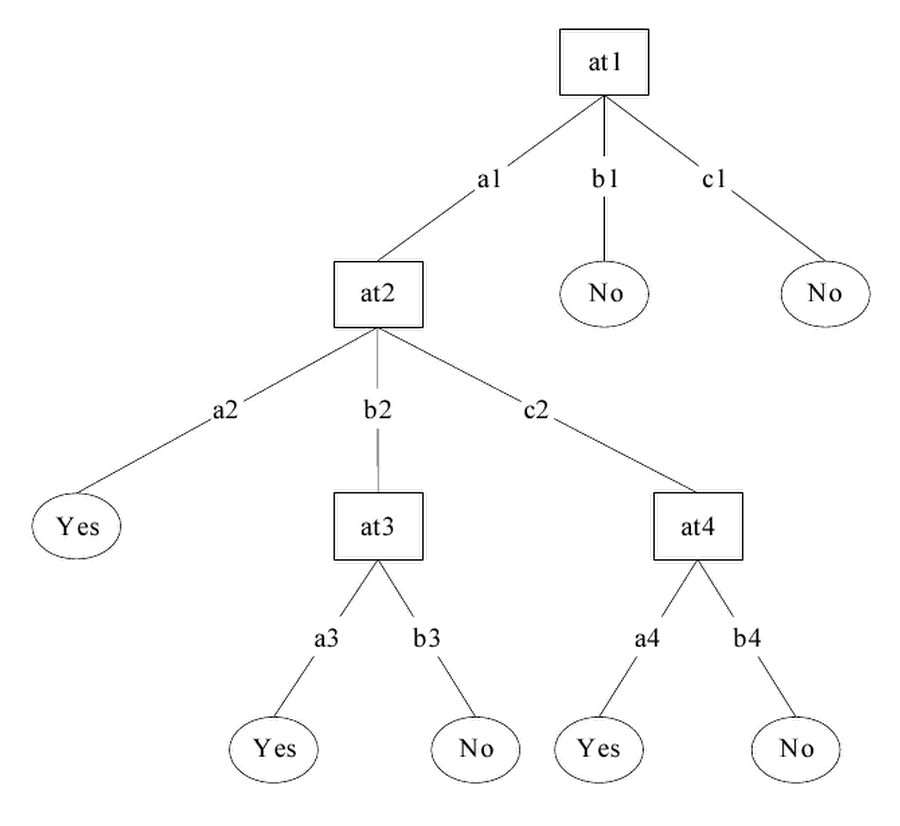
\includegraphics[scale=0.5]{img/decision_tree.png}
		\caption{Príklad jednoduchého rozhodovacieho stromu.}
		\label{img:decision_tree}
	\end{center}
\end{figure}
Ako príklad použijeme rozhodovací strom z obrázku \ref{img:decision_tree}, kde vstupom by bol príklad kde at1 = a1, at2 = b2, at3 = a3 a at4 = a4, algoritmus by zaradil tento príklad postupne do vrcholov at1, at2 a nakonieco do at3 kde by klasifikoval tento príklad ako pozitívny (reprezentovaný hodnotou ``Yes``). Problém zkonštruovania optimálneho rozhodovacieho stromu je NP-úplný problém a preto teoretici hľadali efektívnu heuristiku na zkonštruovanie skoro optimálnych rozhodovacích stromov.\par
Atribút, ktorý najlepšie rozdeluje trénovacie dáta sa nachádza v koreni stromu. Existuje veľa metód na hladanie atribútu, ktorý najlepšie rozdeľuje trénovacie dáta ale väčšina štúdií dospelo k názoru, že neexistuje jedna najlepšia metóda\cite{decision_trees}. Napriek tomu porovnanie individuálnych metód môže byť dôležité pri rozhodovaní, ktorú metriku chceme použiť pre danú dátovú množinu. Rovnaký postup sa potom opakuje na každej časti rozdelených dát a tým sa vytvárajú podstromy až pokým sa trénovacie dáta nerozdelia do podmnožiny z rovnakej triedy.\par
Rozhodovacie stromy sami o sebe nie sú až tak silným nástrojom strojového učenia ale ich jednou z najväčších výhod je to, že proces rozhodovanie je dobre čitateľný aj pre netechnického ľudského používateľa.
\subsection{Náhodné lesy}
Náhodné lesy sú populárnym a veľmi efektívnym algoritmom založeným na spojení myšlienok z viacerých modelov, ktorý sa používa na klasifikačné ako aj na regresné problémy. Po prvý krát bol predložený Breimanom \cite{8}.\par
Algoritmus náhodných lesov je spojením ideí rozhodovacích stromov a tzv. vrecovania (Bagging). Idea vrecovania sa využíva na náhodnu selekciu atribútov podľa ktorej sa vytvorí množstvo rozhodovacích stromov z kontrolovanou varianciou. Každý rozhodovací strom v tomto modele vystupuje ako základný klasifikátor na určenie triedy daného príkladu. Potom ako každý strom samostatne klasifikuje daný príklad výsledná klasifikovaná trieda sa predikuje pomocou väčšinového hlasovania jednotlivých zakladných rozhodovacích stromov.
Obrázok \ref{img:rf_workflow} ilustruje spôsob fungovania algoritmu náhodných lesov a proces algoritmu je interpretovaný nasledovne:
\begin{enumerate}
  \item Z trénovacej množiny, ktorá ma \textit{n} príkladov a \textit{m} atribútov vyber vzorku podľa idei vrecovania.
  \item Pre každú vzorku, vytvor rozhodovací strom s nasledovnou modifikáciou: vyber náhodnú podmnožinu atribútov v každom vrchole stromu a následne nájdi najlepšie rozdelenie podľa atribútov.
  \item Opakuj vyššie uvedené kroky až kým nie je vytvorených počet dopredu určených stromov.
  \item Pošli testovaciu dátovú množinu do náhodného lesu a zagreguj výstupy z jednotlivých rozhodovacích stromov. Klasifikačným výsledkom je výsledok väčšinového hlasovania jednotlivých rozhodovacích stromov.
\end{enumerate}
\begin{figure}[H]
	\begin{center}
		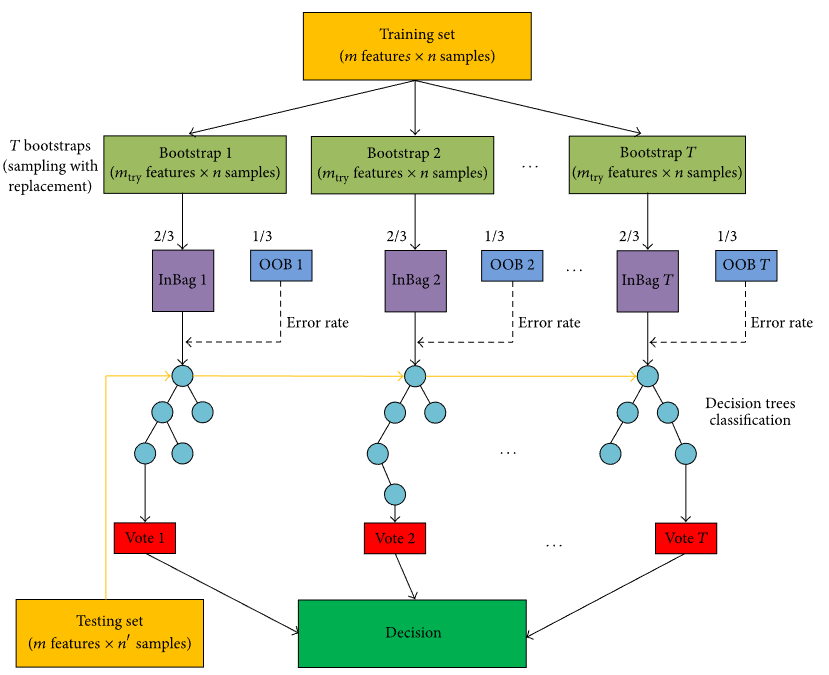
\includegraphics[scale=0.6]{img/rf_workflow.png}
		\caption{Ukážka fungovania algoritmu náhodných lesov.}
		\label{img:rf_workflow}
	\end{center}
\end{figure}
\subsection{Support Vector Machine}
Algoritmy SVM fungujú na základe akéhosi ``zvyšku`` od oboch strán nadroviny, ktorá rozdeľuje dve triedy v dátach. Maximalizovaním tohto zvyšku a teda vytvorenie najväčšej možnej vzdialenosti medzi rozdeľovacou nadrovinou a dátovými bodmi na oboch stranách bolo dokázané, že znižuje horné ohraničenie očakávanej generalizačnej chyby.\par
V prípade kedy sú dáta lineárne separovateľné, potom ako algoritmus nájde optimálnu rozdeľovaciu nadrovinu, dátové body, ktoré ležia na jej zvyšku sa nazývajú bodmi podporných vektorov a riešenie je reprezentované ako lineárna kombinácia iba týchto bodov (obr. \ref{img:svm}). Ostatné dátové body nie sú brané do úvahy. Z toho vyplýva, že zložitosť takých to modelov nie je závislá od počtu charakteristík, ktoré sa vyskytujú v dátovej množine. Počet podporných vektorov vybraných algoritmami SVM je zvyčajne malý. Práve kvôli tomuto sú SVM algoritmy veľmi vhodné na riešenie úloh učenia, kde počet charakteristík je vysoký v pomere ku počtu trénovacích príkladov.\par
\begin{figure}[H]
	\begin{center}
		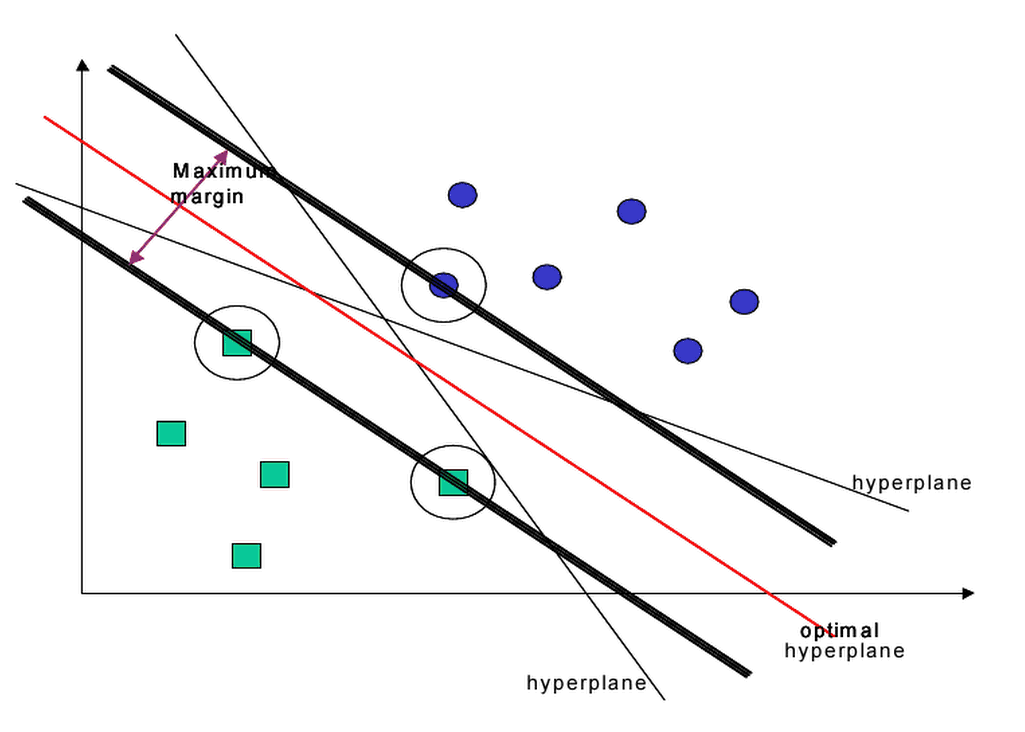
\includegraphics[scale=0.3]{img/svm.png}
		\caption{Ukážka algoritmu SVM.}
		\label{img:svm}
	\end{center}
\end{figure}
Napriek tomu, že maximálny zvyšok dovoľuje algoritmom SVM vybrať spomedzi viacerých kandidátaov nadrovín, pre mnohé dátové množiny tieto algoritmy niesú schopné nájst hociakú rozdelovaciu nadrovinu, pretože dáta obsahuju  príklady, ktoré sú nesprávne zaradené do triedy. Tento problém sa dá riešiť použitím tzv. mäkkým zvyškom, ktorý pripúšťa aj nejaké nesprávne zaradené trénovanie príklady \cite{veropoulos1999}.\par
Väčšina problémov z reálneho sveta poskytuje nerozdelitené dáta, pre ktoré neexistuje nadrovina, ktorá úspešne separuje pozitívne trénovacie príklady od negatívnych. Ďaľšou možnosťou ako tento problém riešiť je tá, že namapujeme dáta do priestoru vyššej dimenzie a definujeme rozdelujúcu nadrovinu v ňom. Tento priestor vyššej dimenzie sa nazýva priesor vlastností (feature space), kdežto priestor, v ktorom sú tréningové príklady voláme vstupný priestor. 
Ak si vhodne zvolíme priestor vlastnotí, tak že má dostatočne vysokú dimenzionalitu, tak vieme rozdeliť hociakú konzistentnú trénovaciu množinu. Lineárna separácia v priestore vlastností korešponduje nelinearnemu rozdeleniu vo pôvodnom priestore vstupov.\par
Ak vhodným spôsobom namapujeme vstupné trénovacie príklady do priestoru vyššej dimenzionality (možno aj nekonečnej), tak trénovací algoritmus záleží len na skalárnom súčine jednotlivých príkladov v našom novom priestore vlastností, teda na funkciách, ktoré majú formu $ \Phi$ (\textit{$x_i$}) $\cdot\ \Phi$( \textit{$x_j$}) . Ak by existovala ``kernelová funkcia`` K taká, že K(\textit{$x_i$}, \textit{$x_j$}) = $\Phi$ (\textit{$x_i$}) $\cdot\  \Phi$(\textit{$x_j$}), tak by trénovací algoritmus potrebovali použiť len K a nikdy by sme nepotrebovali explicitne určit $\Phi$. Teda, kernely sú špeciálnym typom funkcíí. ktoré nám umožňujú počítať skalárne súčiny priamo v priesotre vlastností, bez toho aby sme vykonávali nejaké mapovanie \cite{kernels}. Napokon, keď sa oddeľujúca nadrovina vytvorí, tak kernelová funkcia slúži na namapovanie nových bodov do priestoru vlastností na účel ich klasifikácie.
\subsection{Neurónové siete ako klasifikátor}
Viacvrstvová neurónová sieť pozostáva z veľkého množstva jednotiek (neurónov) spojených dokopy do jedného vzoru (obr. \ref{img:mlp}). Neuróny v sieti sú zvyčajne rozdelené na tri druhy:
\begin{enumerate}
  \item vstupné neuróny - dostávajú informáciu, ktorá má byť spracovaná
  \item výstupné neuróny - výsledky spracovávania informácií sa nachádzajú tu
  \item skryté neuróny - neuróny medzi vstupnou a výstupnou vrstvou
\end{enumerate}
\begin{figure}[H]
	\begin{center}
		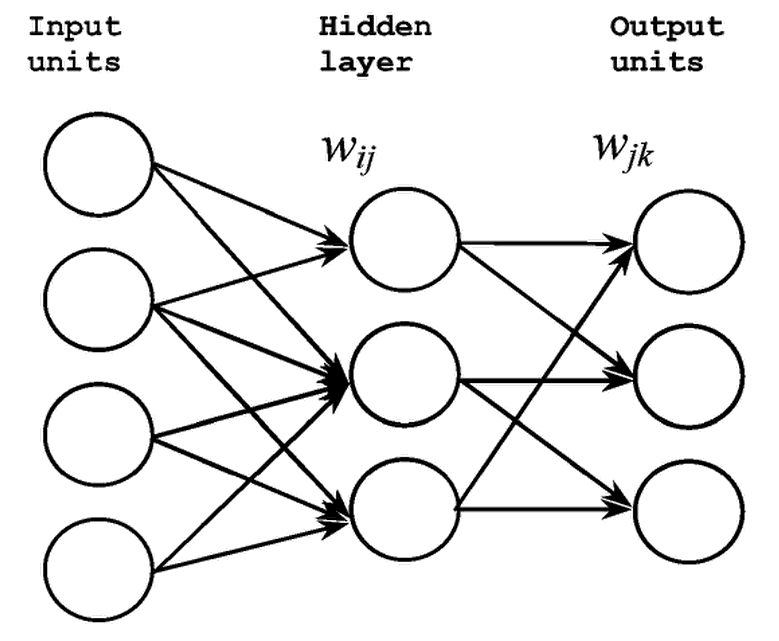
\includegraphics[scale=0.4]{img/mlp.png}
		\caption{Viacvrstvový perceptron.}
	\label{img:mlp}
	\end{center}
\end{figure}
\par Dopredné neurónové sieťe (obr. \ref{img:mlp}) dovoľujú signálu postupovať len vpred, zo vstupnej vrstvy na výstupnú. Najprv je neurónová sieť natrénovaná na označených dátach aby sa určilo mapovanie zo vstupu na výstup. Následne sa váhy na prepojeniach medzi neurónmi zafixujú a potom sa  neurónová sieť používa na klasifikáciu novej dátovej množiny.\par
Vo všeobecnosti, správne určiť veľkosť skrýtej vrstvy je problém, pretože ak podhodnotíme počet neurónov môže to viesť k slabej aproximícii a schopnosti generalizovať. Na druhej strane ak počet neurónov na skrytej vrstve nadhodnotíme toto môže viesť k pretrénovaniu a taktiež to môže znáročniť hľadanie globálneho optima.\par
Neurónové siete závisia na troch hlavných aspektoch, na vstupe a aktivačných funkciách každého neurónu, achitektúre siete a váhach medzi každym spojením neurónov. Vzhľadom na to, že prvé dva aspekty sú fixné tak, správanie neurónovej siete je definované jej aktuálnymi hodnotami váh. Na začiatku trénovacieho procesu neurónovej siete sa váhy nastavia náhodne a následne sa opakovane pošlú príklady z trénovacej množiny neurónovej sieti na vstup. Jednotlivé atribúty trénovacieho príkladu sa pošlú na jednotlivé neuróny na vstupnej vrstve a následne sa výstup neurónovej siete porovná s výsledkom, ktorý sme chceli dosiahnuť pre daný trénovací príklad. Potom sa každá váha neurónovej siete trosku poupraví tak aby sa jej výstup priblížil k výsledku, ktorý sme chceli dosiahnuť na danom trénovacom príklade. Existuje viacero algoritmov ako môžeme neurónovú sieť trénovať\cite{nn_training}. Najznámejším a najpoužívanejším učiacim algoritom na odhadnutie hodnôt váh neurónovej siete je algoritmus spätnej propagácie (Back Propagation) \cite{backprop}.\par
Hlavnou nevýhodou neurónových sietí je, oproti rozhodovacím stromom, že nevieme dobre argumentovať o ich výstupoch. Neurónové siete sú často krát nazývané aj čiernou skrinkou, pretože vidíme len vstupy a výstupy. Procesy vo vnútri tejto ``skrinky`` sa ťažko vysvetľujú.
